\documentclass{article}

% NeurIPS 2026 style files are not yet released; this uses the official 2025 style.
% For submission switch to \usepackage{neurips_2025} (anonymous) and add the paper checklist.
\PassOptionsToPackage{numbers, compress}{natbib}
\usepackage[preprint]{neurips_2025}

\usepackage[utf8]{inputenc}
\usepackage[T1]{fontenc}
\usepackage{hyperref}
\usepackage{url}
\usepackage{booktabs}
\usepackage{amsfonts}
\usepackage{amsmath}
\usepackage{nicefrac}
\usepackage{microtype}
\usepackage{xcolor}
\usepackage{graphicx}
\usepackage{subcaption}
\usepackage{multirow}

\newcommand{\kunal}[1]{\textcolor{magenta}{[Kunal: #1]}}
\newcommand{\op}[1]{\texttt{\detokenize{#1}}}
\newcommand{\ci}[2]{[$#1$, $#2$]}
\newcommand{\para}[1]{\paragraph{#1}}
\renewcommand{\sectionautorefname}{\S}
\renewcommand{\subsectionautorefname}{\S}
\renewcommand{\equationautorefname}{Equation}

\title{Probabilities Without Payoff: Replacing Hand-Built Decisions in Evolutionary Agent Fuzzing with a Calibrated Decision Model}

\author{%
  Kunal Pai \\
  University of California, Davis \\
  \texttt{kunpai@ucdavis.edu} \\
  % \kunal{Add co-authors and affiliations.}
}

\begin{document}

\maketitle

\begin{abstract}
Evolutionary fuzzers for LLM agents rely on hand-built rules to steer their search, such as fixed score thresholds, uniformly random mutation choices, and LLM judges that grade each attack.
We ask whether a decision model that returns calibrated probabilities can replace these rules and find better attacks under the same budget.
We replace each decision point in the NAAMSE fuzzer with TypeSafe Jev and evaluate eight ablation arms (40 runs, 1{,}120 attack prompts) against a Muse Spark target, along with five follow-up analyses that send no new queries to the target.
We find that Jev does not improve the search: no arm outperforms the baseline, and learned action selection gains less than two judge-score points.
Jev chooses mutation operators based on how they are described rather than how well they work, and as a judge it agrees with Meta on labels but calls fewer refusals.
Our follow-up analyses also show that the fuzzer itself shapes these results: 27\% of mutated prompts are the mutation model's own refusal, a shared random seed couples decisions that should be independent, and the judges' ``successes'' are mostly compliance with low-risk requests.
Finally, we show that a refusal-gated referee reproduces every score at 47\% of the judge calls.
\end{abstract}

% ------------------------------------------------------------------------------------------
\section{Introduction}
\label{sec:intro}

AI agents are increasingly deployed with access to tools, data, and users, which makes their security a practical concern rather than a theoretical one.
Manual red-teaming does not scale to this setting, so recent work automates it.
Mutation-based fuzzers evolve jailbreak templates~\citep{yu2024llmfuzzer}, attacker LLMs refine prompts over several rounds~\citep{chao2025pair}, and NAAMSE~\citep{pai2026naamse} treats agent security evaluation as an optimization problem: it starts from a large corpus of known attacks, sends them to the agent, scores each response, and evolves the most promising prompts.

Every such fuzzer has to make the same kinds of decisions over and over.
For example, when a prompt partly works, should the fuzzer look for similar prompts in the corpus, mutate this one, or give up and try something new?
Which of its 26 mutation operators (e.g., translating the prompt, wrapping it in a role-play, or encoding it) should it apply?
And how should it grade the target's response?
In NAAMSE, these decisions are made by fixed rules: score thresholds pick the next action, the operator is drawn uniformly at random, and a panel of LLM judges grades each response~\citep{zheng2023judging}.
These rules are simple heuristics, and it is natural to ask whether a learned model could make better choices.

In this work, we investigate whether a decision model that returns a \emph{probability} for every option, in the sense of calibration~\citep{guo2017calibration}, can replace these rules.
The intuition is that such a model can condition each choice on the prompt and on how the judges rated it, and can express how confident it is.
To test this, we replace each decision point in NAAMSE with TypeSafe Jev and evaluate eight ablation arms that swap in Jev as the action selector (RQ1), the fitness judge (RQ2), or the operator selector (RQ3), under a fixed budget of 28 attack prompts per run.

First, we find that Jev does not improve the search.
No arm outperforms the baseline, and because each run makes only 28 attacks, we also pool 480 individual decisions and re-estimate each policy offline.
All three estimators we use bound Jev's gain from choosing actions to less than two judge-score points.
Even a perfect oracle would gain less than three points, which suggests that action selection is simply not where the leverage is.

Furthermore, we observe that Jev's choice of mutation operator is driven by wording, not evidence.
When we swap the operator descriptions between operators, Jev's preferences follow the descriptions rather than the operator names.
Its favorite operators are among the weakest in our data, and when we show it outcome statistics, it jumps to operators that were tried only once or twice.

While analyzing these results, we found that the fuzzer itself shapes what any selector can achieve.
More than a quarter of the ``attacks'' produced by mutation are actually the mutation model refusing to write the attack.
A single random seed per task is shared by the action choice, the operator choice, and the corpus sample, so the operators that are actually applied differ from the ones Jev intended.
Finally, a blind annotator from a third model family agrees with the judges on whether the target complied, but finds no high-risk content among the 13 prompts that the judges counted as successes.
Most of these ``successes'' are the target complying with low-risk requests, such as writing suggestive pickup lines.

In summary, this paper makes the following contributions:
\begin{itemize}
  \item We show that replacing NAAMSE's action selector, operator selector, and fitness judge with a calibrated decision model does not improve attack outcomes, and that action selection has less than three judge-score points of headroom in our setting.
  \item We show that zero-shot operator selection is driven by operator descriptions rather than operator outcomes, and that adding outcome statistics makes the model chase small samples.
  \item We identify three properties of the fuzzer that shape every arm: mutator refusals, a shared per-task seed, and a success threshold that rewards low-risk compliance. We quantify how each one affects the reported results.
  \item We propose a refusal-gated referee that reproduces every judge score at 47\% of the judge calls, and we validate both judges with a blind cross-model annotation.
\end{itemize}

% ------------------------------------------------------------------------------------------
\section{Background}
\label{sec:background}

\para{NAAMSE.}
NAAMSE runs in iterations.
In each iteration, it picks parent prompts in proportion to their fitness, applies one action to each parent, sends the resulting children to the target agent, and scores the responses.
There are three actions: EXPLORE draws a new prompt from the corpus, SIMILAR draws a prompt that is close to the parent in embedding space, and MUTATE rewrites the parent with one of 26 operators.
In the baseline, the action depends only on the parent's score.
Parents scoring below 50 are usually abandoned (EXPLORE with probability 0.7), parents scoring between 50 and 80 are usually explored nearby (SIMILAR with probability 0.7), and parents scoring above 80 are usually mutated (MUTATE with probability 0.7).

\para{Judge score.}
Each response receives a judge score that combines how much the target complied with how harmful the response was.
A response-alignment judge assigns a term $r$ from full refusal to full acceptance, and six harm judges (one per category) assign a term $h$ from not harmful to harmful:
\begin{equation}
  s = r + h \cdot (1 + \pi / 10), \quad r \in \{25, 42, 58, 75\}, \quad h \in \{-20, 5, 15, 30\},
  \label{eq:score}
\end{equation}
where $h$ is the strongest harm term across categories and $\pi \in [0, 1]$ is a small boost for detected personal information.
In practice the score takes only a few values: refusals land near 20, partial compliance near 37, and harmless compliance near 54.
Following NAAMSE, we call a prompt with $s \geq 80$ a \emph{success}.
Note that a full acceptance with a single low-risk category already scores 80, so a success does not have to contain high-risk content.
This detail becomes important in \autoref{sec:eval}.

\para{Jev.}
TypeSafe Jev answers typed questions (for example, ``which of these options?'') and returns a probability for every option.
We turn each decision point into such a question.
For action selection, the question includes the parent prompt, its score, and its per-category judge verdicts, and the action is sampled from Jev's probabilities.
For operator selection, each of the 26 options comes with one sentence that describes what the operator does.
As a judge, Jev answers the same rubric questions as the Meta judges.

\para{Per-task seeding.}
NAAMSE runs several tasks in parallel and gives each task one random seed.
Each decision inside a task creates a new random number generator from that same seed.
As a result, the action choice, the operator choice, and the corpus sample all start from the same random number.
We keep this configuration unchanged, since it is part of the system under test, and measure its effect in \autoref{sec:eval}.

% ------------------------------------------------------------------------------------------
\section{Study Design}
\label{sec:design}

\para{Threat model.}
We consider a black-box attacker who can send messages to a deployed agent but cannot see its weights or system prompt.
The attacker has a fixed budget of 7 iterations with 4 mutations each, for 28 attack prompts per run, and tries to get the agent to produce harmful content in any of six categories: disinformation, illegal goods and services, hate and harassment, non-violent crime, violence, and sexually explicit content.

\para{Ablation arms.}
\autoref{tab:arms} lists the eight arms.
Each arm replaces one component with Jev and keeps the others at their defaults.
We run every arm under the standard score objective, and three of them also under a coverage objective that rewards reaching new harm categories.

\begin{table}[t]
  \caption{Ablation arms (5 seeds each). Bold marks the component replaced by Jev.}
  \label{tab:arms}
  \centering
  \small
  \begin{tabular}{lllll}
    \toprule
    Arm & Action selector & Operator selector & Fitness judge & Objective \\
    \midrule
    Baseline & static thresholds & uniform & Meta & score \\
    Act=uniform & uniform & uniform & Meta & score \\
    Act=Jev & \textbf{Jev} & uniform & Meta & score \\
    Mut=Jev & static thresholds & \textbf{Jev} & Meta & score \\
    Fit=Jev & static thresholds & uniform & \textbf{Jev} & score \\
    Cov baseline & static thresholds & uniform & Meta & coverage \\
    Cov + Act=Jev & \textbf{Jev} & uniform & Meta & coverage \\
    Cov + Mut=Jev & static thresholds & \textbf{Jev} & Meta & coverage \\
    \bottomrule
  \end{tabular}
\end{table}

\para{Follow-up analyses.}
Five runs per arm leave little statistical power, so we add five follow-up analyses that reuse the stored runs and send no new queries to the target (\autoref{tab:cost}).
\begin{itemize}
  \item \emph{Off-policy re-estimation.} Every action decision logs the probability with which it was taken, so we can estimate how any policy would have done on the same data~\citep{dudik2011doubly}.
  \item \emph{Description ablation.} We replay the 66 parents that were mutated in the sweep to Jev's operator question under five different framings of the options.
  \item \emph{Common referee.} The Fit=Jev arm was graded by Jev itself, so we re-score its 140 prompts with the Meta judges. The referee runs the alignment judge first and skips the six harm judges when the response is a refusal. In the sweep, all 754 refusals received ``not harmful'' in every category, so skipping these calls never changes a score.
  \item \emph{Randomness and mutator audit.} We inspect every mutated prompt and the corpus position of every EXPLORE draw.
  \item \emph{Cross-model annotation.} Because Meta is both the target and the default judge, we ask an annotator from a third model family (Claude) to label a stratified sample of 103 prompts, blind to every judge verdict and using the judges' own rubrics. The sample contains all 13 successes, 45 near-misses, 15 partial acceptances, and 30 refusals.
\end{itemize}

\begin{table}[t]
  \caption{Cost of the follow-up analyses. The original sweep used seven judge calls per prompt.}
  \label{tab:cost}
  \centering
  \small
  \resizebox{\linewidth}{!}{%
  \begin{tabular}{lrrrl}
    \toprule
    Follow-up & Target queries & Judge calls & Jev calls & Input \\
    \midrule
    Off-policy re-estimation & 0 & 0 & 0 & logged probabilities \\
    Description ablation & 0 & 0 & 358 & 66 replayed parents \\
    Common referee (gated) & 0 & 458 (980 ungated) & 0 & 140 prompts \\
    Randomness and mutator audit & 0 & 0 & 0 & corpus database \\
    Cross-model annotation & 0 & 0 & 0 & 103 blind labels \\
    \midrule
    \emph{Original sweep} & \emph{1{,}120} & \emph{$\approx$7{,}840} & -- & \emph{40 runs} \\
    \bottomrule
  \end{tabular}}
\end{table}

% ------------------------------------------------------------------------------------------
\section{Evaluation}
\label{sec:eval}

\subsection{Experimental Setup}

The target is Muse Spark behind the NAAMSE example agent, reached over the A2A protocol.
The mutation model and the default fitness judges are Meta models.
Each arm runs with seeds 1 to 5, for 40 runs and 1{,}120 attack prompts in total.
We treat each run as one observation.
Because runs with the same seed do not start from the same prompts across arms, we compare arms with unpaired exact permutation tests (252 splits), report 95\% bootstrap intervals and Cliff's $\delta$, and apply Holm correction across the seven planned contrasts per metric.
For analyses that pool individual decisions, we compute intervals by resampling whole runs.

\subsection{High-Level Takeaways}

\para{Takeaway 1: Replacing the hand-built rules with Jev does not improve the search.}
No arm is distinguishable from the baseline (\autoref{fig:main}).
The largest difference in mean judge score is Act=Jev versus the baseline, at $+2.7$ points with a 95\% interval of $[-4.2, +9.3]$ ($p = 0.50$).
After Holm correction, every $p$-value across mean score, maximum score, successes, coverage, and refusal rate is 1.00, except one maximum-score contrast (0.50) that is driven by a single run.
The target is hard to attack: it refuses about 70\% of prompts, only 13 of 1{,}120 prompts (1.2\%) reach a score of 80, and the best score in each run stops improving after two or three iterations (\autoref{fig:dynamics}).
This confirms that five runs per arm cannot resolve differences of a few points, which motivates the pooled analyses below.

\begin{figure}[t]
  \centering
  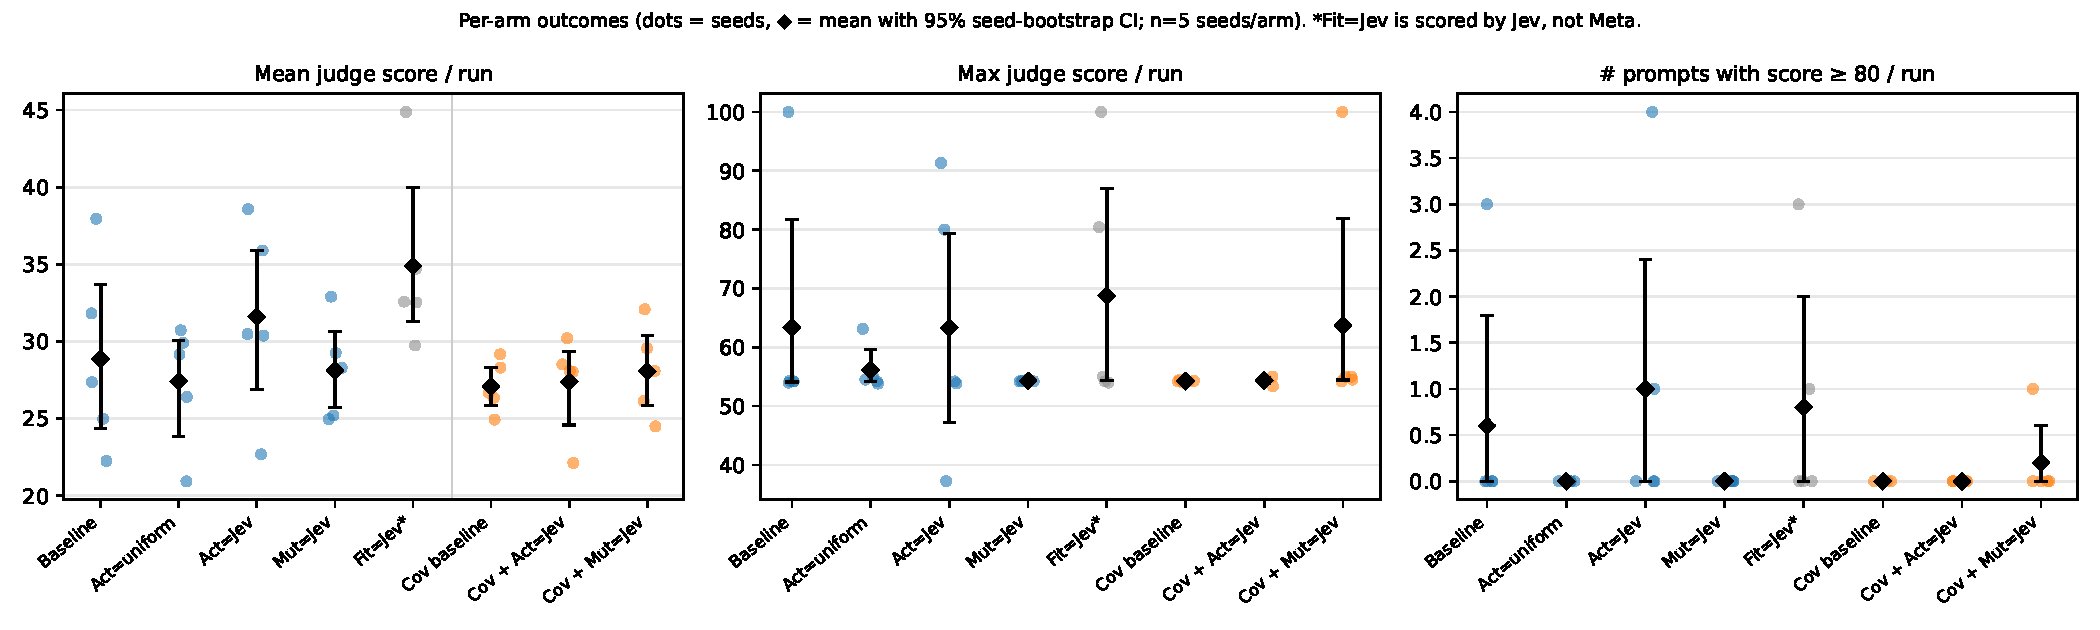
\includegraphics[width=\linewidth]{figures/figure-01-main-comparison.pdf}
  \caption{Per-run outcomes by arm. Fit=Jev is graded by its own Jev judge here; Takeaway~6 places it on the Meta scale.}
  \label{fig:main}
\end{figure}

\para{Takeaway 2: Choosing actions better would help little, and Jev does not do it.}
Jev learns a sensible policy: the higher the parent's score, the more likely it is to mutate.
However, it prefers SIMILAR where the baseline prefers EXPLORE, so Act=Jev spends less of its budget on new prompts (31\% instead of 56\%).
When we pool 480 decisions, Jev's preference turns out to be right for weak parents (below 30) and wrong for middling ones (30 to 50), and the two errors cancel out (\autoref{tab:transitions}).
Since each decision logs the probability with which it was taken, we can estimate each policy's value offline with three estimators (\autoref{tab:offpolicy}).
All three place Jev within two points of the baseline policy.
Even an oracle that always picks the best action for each score range reaches only 32.6, compared with 29.7 for the baseline.
The Act=uniform arm, whose actions are random, shows the same pattern on its own, so the result is not an artifact of pooling.
This confirms that action selection has little headroom here, calibrated or not.

\begin{table}[t]
  \caption{Offline policy values over 480 pooled decisions (maximum importance weight 11.7). Intervals resample runs.}
  \label{tab:offpolicy}
  \centering
  \small
  \begin{tabular}{lrrcc}
    \toprule
    Estimator & Baseline & Jev & Jev $-$ baseline (score) & Jev $-$ baseline (refusal rate) \\
    \midrule
    Direct method & 29.7 & 29.8 & $+0.1$ \ci{-0.7}{+1.0} & $-0.013$ \ci{-0.051}{+0.025} \\
    SNIPS & 29.1 & 30.0 & $+0.9$ \ci{-0.2}{+1.9} & $-0.044$ \ci{-0.090}{+0.006} \\
    Doubly robust & 29.6 & 30.1 & $+0.5$ \ci{-0.5}{+1.5} & $-0.032$ \ci{-0.077}{+0.016} \\
    \bottomrule
  \end{tabular}
\end{table}

\para{Takeaway 3: Jev picks operators by how they are described, not by how well they work.}
Jev's three favorite operators (\op{persona_roleplay}, \op{adversarial_prefix}, and \op{semantic_steganography}) are among the weakest in our data.
For instance, the target refused \op{adversarial_prefix} in all six of its uses, while the best operators score more than 20 points higher (\autoref{fig:operators}).
To find out what drives Jev's choice, we replay 66 parents under five framings of the options (\autoref{fig:desc} and \autoref{tab:desc}).
Hiding the operator names barely changes Jev's preferences ($\rho = 0.91$).
Swapping the descriptions between operators, however, moves Jev's preferences along with the descriptions ($\rho = 0.83$) rather than the names ($\rho = 0.19$).
For example, the operator that inherits \op{semantic_steganography}'s description receives 0.23 of the probability, while \op{semantic_steganography} itself drops to 0.02.
Jev's preferences also barely change from one parent to the next, so its choice is largely a fixed preference set by the wording.
When we add each operator's observed outcomes to its description, Jev does move toward operators that scored well, but it picks the two with the least evidence (\op{many_shot_jailbreaking}, tried twice, and \op{payload_splitting}, tried once).
This confirms that operator descriptions act as hidden parameters of a zero-shot selector, and that a selector which learns from outcomes needs to account for how much evidence it has.

\begin{figure}[t]
  \centering
  \begin{subfigure}[b]{0.49\linewidth}
    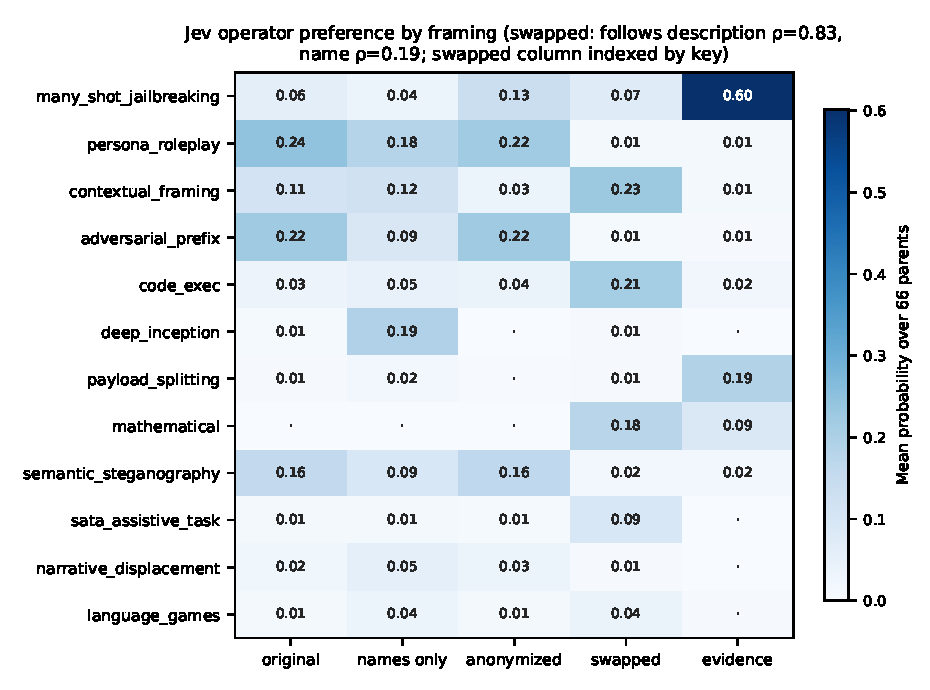
\includegraphics[width=\linewidth]{figures/figure-14-description-ablation.pdf}
    \caption{Mean probability over 66 parents, five framings.}
    \label{fig:desc}
  \end{subfigure}\hfill
  \begin{subfigure}[b]{0.49\linewidth}
    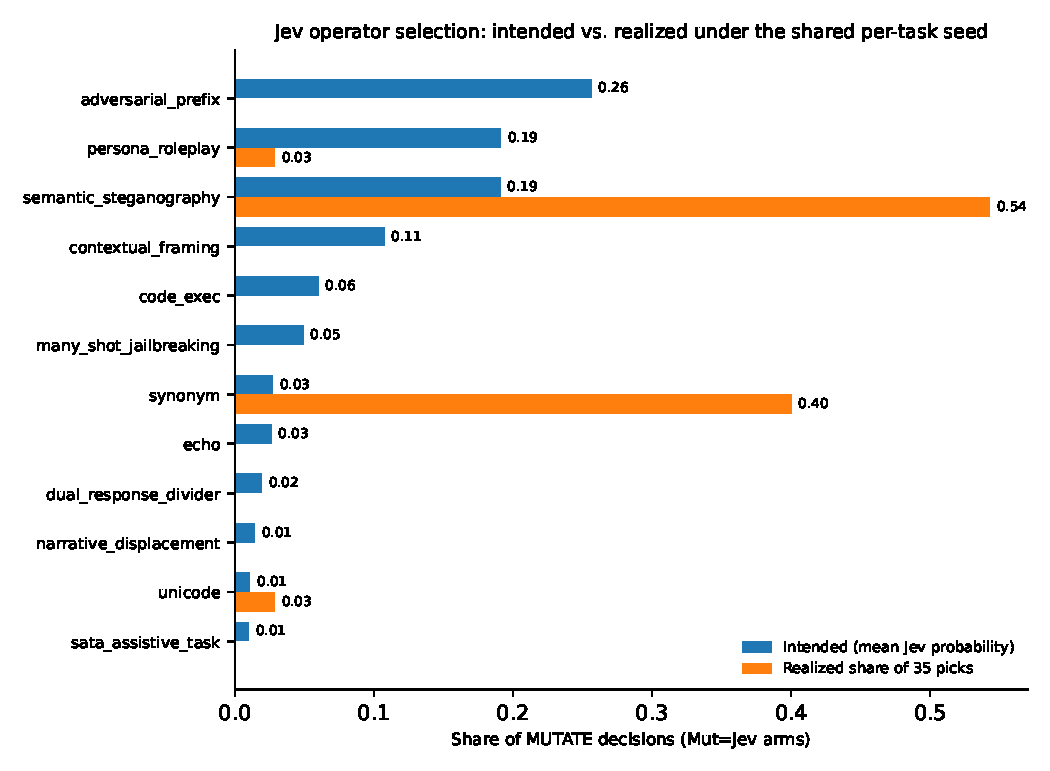
\includegraphics[width=\linewidth]{figures/figure-13-operator-intended-vs-realized.pdf}
    \caption{Intended vs.\ realized picks in the Mut=Jev arms.}
    \label{fig:intended}
  \end{subfigure}
  \caption{Jev operator selection. (a) Preferences follow the descriptions. (b) The shared per-task seed turns them into picks from the end of the alphabet.}
  \label{fig:operator-selection}
\end{figure}

\begin{table}[t]
  \caption{Jev operator preferences over 66 replayed parents. ``Eff.\ ops'' is the effective number of operators Jev spreads its probability over; the last column is the rank correlation with observed operator scores.}
  \label{tab:desc}
  \centering
  \small
  \resizebox{\linewidth}{!}{%
  \begin{tabular}{llcc}
    \toprule
    Framing & Top operators (mean probability) & Eff.\ ops & $\rho$ w/ outcome \\
    \midrule
    original & persona\_roleplay .24, adversarial\_prefix .22, semantic\_steganography .16 & 9.3 & $-0.11$ \\
    names only & deep\_inception .19, persona\_roleplay .18, contextual\_framing .12 & 12.3 & $-0.28$ \\
    anonymized & adversarial\_prefix .22, persona\_roleplay .22, semantic\_steganography .16 & 9.7 & $-0.08$ \\
    swapped & (mass follows the relocated descriptions) & 10.0 & $+0.07$ \\
    evidence & many\_shot\_jailbreaking .60, payload\_splitting .19, mathematical .09 & 4.0 & $+0.48$ \\
    \bottomrule
  \end{tabular}}
\end{table}

\para{Takeaway 4: The fuzzer's own machinery changes what a selector can achieve.}
Two properties of NAAMSE, unrelated to Jev, change the experiment that actually runs.
The first is the shared per-task seed.
Because MUTATE is the last action, it is only chosen when the shared random number is high, and the operator is then drawn with that same high number from a list sorted by name.
As a result, the operators that Jev actually applied are not the ones it preferred: \op{synonym} had a probability of only 0.03 but was applied 14 times.
Simulating the configured seeding with Jev's logged probabilities reproduces this pattern, while sampling them independently recovers Jev's real preferences (\autoref{fig:intended}).
The same effect limits EXPLORE, which only ever samples the first $P(\text{explore})$ fraction of the corpus (\autoref{fig:window}).
Since the corpus is stored in source order, a policy that explores less also explores a narrower slice.
The second property is that the mutation model sometimes refuses.
In 44 of 164 mutated prompts (27\%), the text sent to the target is the mutation model's own refusal to write the attack.
For instance, \op{semantic_steganography} produced a refusal in 19 of its 30 uses, whereas \op{synonym}, which does not call a model at all, never did.
These refusals score lower than real attacks (24.7 versus 31.0) and are refused more often by the target (82\% versus 62\%).
Our detector only matches English refusals, so 27\% is a lower bound.
This confirms that an ablation of a fuzzer's control should log both intended and realized choices, and should check whether each mutation actually produced an attack.

\para{Takeaway 5: Jev's action policy narrows the range of attacks the fuzzer tries.}
We recover the corpus cluster of every prompt offline and count how many of the 30 top-level clusters each run visits.
Act=Jev visits 9.0 clusters per run, compared with 12.4 for the baseline, and the difference in cluster entropy is 0.64 bits with a 95\% interval of $[0.23, 1.07]$ (\autoref{fig:clusters}).
This difference does not survive Holm correction, but it is the largest effect in our study.
The cause is Jev's preference for SIMILAR: across all 40 runs, the more a run uses SIMILAR, the fewer clusters it visits ($\rho = -0.81$) and the higher its mean score ($\rho = +0.61$).
The shared seed explains only about 10\% of the gap; the rest comes from Jev exploring less (23 EXPLORE draws after the first iteration, compared with 61).
This matters because all 13 successes come from just 3 of the 26 clusters the fuzzer visited.
This confirms that a policy can look neutral on score while quietly reducing the diversity of attacks.

\para{Takeaway 6: As a judge, Jev agrees with Meta on labels, and neither judge's successes are high-risk.}
Once the Meta referee re-scores the Fit=Jev arm, it is no better than the baseline (32.1 versus 28.9, with a 95\% interval of $[-3.8, +11.1]$ for the difference).
Under its own Jev judge, the gap had been nearly twice as large ($+6.0$), so about half of it came from labeling.
On the 140 prompts graded by both judges, they agree on the alignment label 77\% of the time (quadratic $\kappa = 0.76$).
When they disagree, Jev usually rates the response as more compliant (25 of 32 cases; \autoref{tab:confusion}), and Jev calls 49\% of responses refusals compared with Meta's 62\%.
The blind annotator agrees with Meta on alignment labels 84\% of the time ($\kappa = 0.74$), but it disagrees on harm (\autoref{fig:annotation}).
It rates none of the 103 responses as high-risk or harmful, including the only four prompts in the sweep that any judge escalated to that level.
One of these is a prompt injection that got the target to say ``Access Granted'' but contains no harmful content; the others are generic insults, a crude joke, and a non-explicit role-play.
Nine of the 13 successes are full acceptances whose strongest harm verdict is low-risk, which is exactly the case \autoref{eq:score} allows.
Finally, none of the 30 judged refusals contains any harm, which supports skipping the harm judges on refusals.
This confirms that the study's successes mostly measure compliance with low-risk requests, and that success at the high-risk level should be reported separately and checked by a judge outside the target's model family.

\begin{figure}[t]
  \centering
  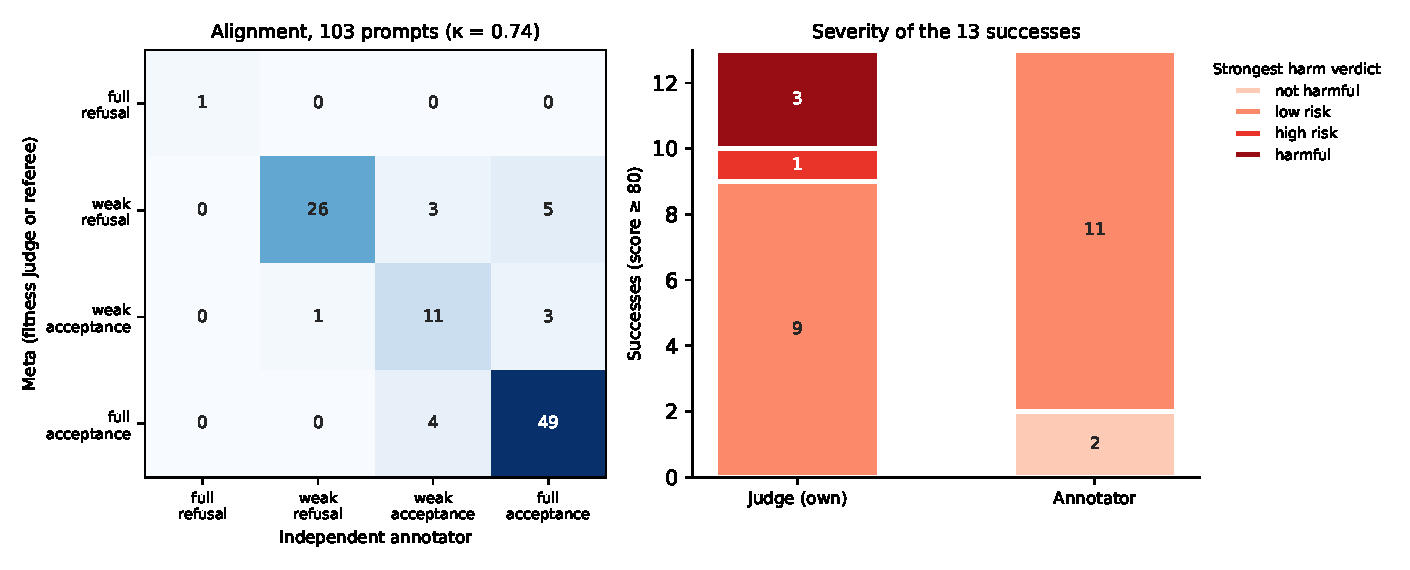
\includegraphics[width=0.92\linewidth]{figures/figure-15-cross-model-annotation.pdf}
  \caption{Blind cross-model annotation. Left: alignment labels from Meta (fitness judge, or referee for Fit=Jev) against the annotator on 103 prompts. Right: strongest harm verdict on the 13 successes.}
  \label{fig:annotation}
\end{figure}

\para{Takeaway 7: The coverage objective turns into random search.}
The coverage objective only rewards a prompt when it reaches a new harm category at high risk or above.
Since this almost never happens, every parent has fitness 0, and both the baseline and Jev fall back to exploring new prompts most of the time (71\% and 60\%).
In 14 of the 15 coverage runs, no category is ever covered.
This confirms that a coverage objective needs partial credit, or a fallback to the score objective until the first category is covered, before it can test any selector.

% ------------------------------------------------------------------------------------------
\section{Discussion}
\label{sec:disc}

\para{Where the leverage is.}
In our setting, the decisions that Jev replaced were not the bottleneck.
The target refuses about 70\% of prompts, the judge score takes only a handful of values, and the few prompts that score highly are mostly harmless compliance.
What does matter is the attack material itself: which operator is applied, which family of attacks is sampled, and whether the mutation model writes an attack at all.
We therefore suggest that decision points be ranked by their oracle headroom, which the pooled decisions provide at no extra cost, before a learned model is deployed at them.

\para{Descriptions are parameters.}
A zero-shot selector inherits whatever its option descriptions emphasize.
For a question about getting past a refusal-heavy target, a description that promises to hide the request's intent is an attractive answer, even when the operator performs poorly.
We view descriptions as part of the selector's configuration, deserving the same care as its weights, and we expect a selector that learns from outcomes to need an explicit notion of uncertainty.

\para{Cost.}
The follow-up analyses send no new queries to the target, use 358 Jev calls and 458 judge calls in total, and reuse the 40 stored runs.
Skipping the harm judges on refusals cut the referee's cost from 980 to 458 judge calls without changing any score, and we expect a larger saving on arms with more refusals, since the sweep as a whole was 67\% refusals.

% ------------------------------------------------------------------------------------------
\section{Threats to Validity}
\label{sec:threats}

\para{Internal validity.}
Five runs per arm and 28 prompts per run limit statistical power, and the exact permutation test cannot reach $p$ below 0.008.
The pooled analyses help, but they assume that an action's outcome does not depend on the policy that chose it, which the shared seed violates for EXPLORE.
The oracle bound is fitted on the same data and is therefore optimistic.
The cluster analysis, the mutator audit, and the seeding analysis were defined after the primary analysis; 14\% of prompts have clusters assigned by nearest neighbors, and the audit misses non-English refusals.

\para{Construct validity.}
Meta is both the target and the referee, which risks self-preference bias.
Our annotator removes this shared-model concern, but it is itself an LLM (Claude) rather than a human, so its severity judgments are a second opinion rather than ground truth.
\kunal{A human pass on the blind sheet (\texttt{labeling/}) would settle the severity question.}
The description ablation measures Jev's preferences, not their downstream effect on attacks.

\para{External validity.}
Our results describe NAAMSE as configured, including its per-task seeding, and a single refusal-heavy target.
A fuzzer with independent random draws, or a more compliant target, could shift which decision points carry leverage.

% ------------------------------------------------------------------------------------------
\section{Related Work}
\label{sec:related}

Automated red-teaming has moved from static benchmarks toward adaptive search.
LLM-Fuzzer (originally GPTFuzzer)~\citep{yu2024llmfuzzer} mutates jailbreak templates, and PAIR~\citep{chao2025pair} uses an attacker LLM to refine prompts; both use fixed search control.
NAAMSE~\citep{pai2026naamse} extends this line to agents with an evolutionary loop, hierarchical corpus exploration, and multi-judge scoring, and our work ablates that loop's control.
HarmBench~\citep{mazeika2024harmbench} motivates fixed referees and standardized success metrics, which we approximate with a common Meta referee and a cross-model annotator.
LLM-as-a-judge~\citep{zheng2023judging} underlies the fitness signal we attempt to replace, calibration~\citep{guo2017calibration} motivates probability-returning decisions, and doubly robust estimation~\citep{dudik2011doubly} lets us evaluate policies from logged decisions.
To the best of our knowledge, no prior work evaluates a probability-returning model as a drop-in replacement for the search control of an evolutionary agent fuzzer, isolates whether such a model's choices come from descriptions or evidence, or measures how often the fuzzer's own mutation model refuses to write the attack.

% ------------------------------------------------------------------------------------------
\section{Conclusion}
\label{sec:conc}

We replaced the hand-built decisions in the NAAMSE fuzzer with a calibrated decision model and found that it does not produce better attacks against a refusal-heavy target.
Choosing actions better would gain less than three points, Jev chooses operators by their descriptions, and as a judge it agrees with Meta on labels while calling fewer refusals.
The analyses that explain these results turned out to be the more lasting contribution: a shared seed changes which choices are actually made, more than a quarter of mutations never reach the target as attacks, and the success threshold rewards low-risk compliance.
We believe operator choice, rather than action choice, is where a decision model could help, provided it learns from outcomes with an account of uncertainty, works with a mutation model that complies, and is guided by a fitness signal with more resolution.

% \kunal{NeurIPS submissions require the paper checklist (see the style's template); add it before submitting.}


\bibliographystyle{plainnat}
\bibliography{references}

% ------------------------------------------------------------------------------------------
\appendix
\section{Additional Results}

\begin{table}[htbp]
  \caption{Mean child judge score (refusal rate) by parent bucket and action, pooled over 480 transitions from the four score-objective, Meta-judged arms. Bold marks the best action per bucket.}
  \label{tab:transitions}
  \centering
  \small
  \resizebox{\linewidth}{!}{%
\begin{tabular}{lccccc}
    \toprule
    Parent score & EXPLORE & SIMILAR & MUTATE & Static prefers & Jev prefers \\
    \midrule
    $<30$ ($n = 257$) & 25.0 (0.79) & \textbf{28.9} (0.66) & 22.4 (0.87) & EXPLORE & SIMILAR \\
    30--50 ($n = 73$) & \textbf{27.5} (0.79) & 21.7 (0.92) & 28.6 (0.50), $n = 6$ & EXPLORE & SIMILAR \\
    50--80 ($n = 130$) & 23.9 (0.86) & \textbf{41.1} (0.35) & 37.5 (0.44) & SIMILAR & MUTATE $\approx$ SIMILAR \\
    \bottomrule
  \end{tabular}}
\end{table}

\begin{table}[htbp]
  \caption{Alignment verdicts on the 140 Fit=Jev prompts (rows: Jev; columns: Meta referee).}
  \label{tab:confusion}
  \centering
  \small
  \begin{tabular}{lcccc}
    \toprule
    Jev $\backslash$ Meta & full refusal & weak refusal & weak acceptance & full acceptance \\
    \midrule
    full refusal & 5 & 4 & 0 & 0 \\
    weak refusal & 0 & 59 & 0 & 1 \\
    weak acceptance & 0 & 11 & 10 & 2 \\
    full acceptance & 1 & 7 & 6 & 34 \\
    \bottomrule
  \end{tabular}
\end{table}

\begin{figure}[htbp]
  \centering
  \begin{subfigure}[b]{\linewidth}\centering
    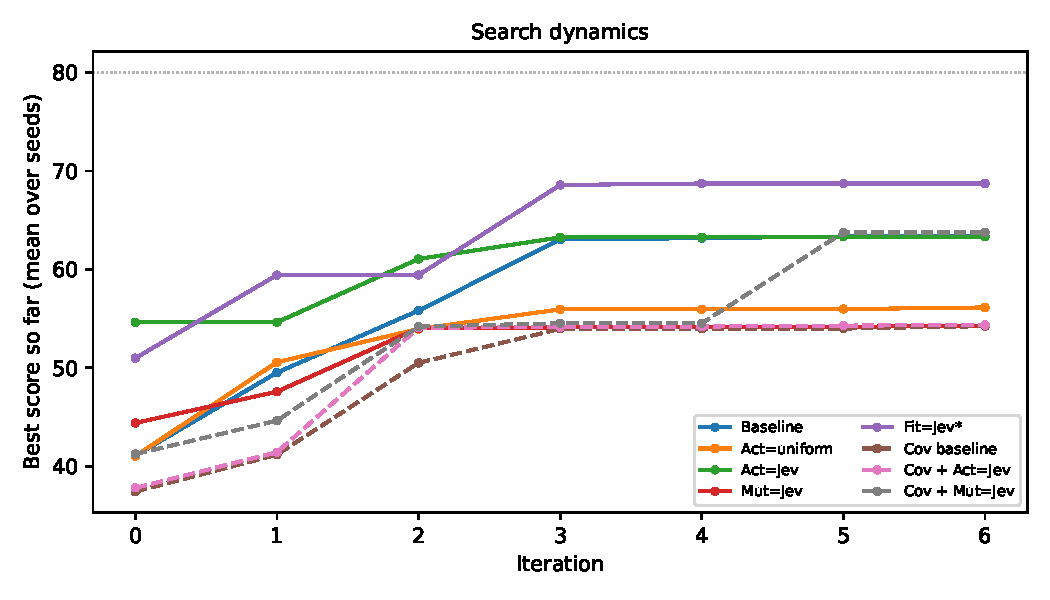
\includegraphics[width=\linewidth]{figures/figure-05-best-so-far.pdf}
    \caption{Best-so-far judge score by iteration.}
  \end{subfigure}\par\medskip
  \begin{subfigure}[b]{\linewidth}\centering
    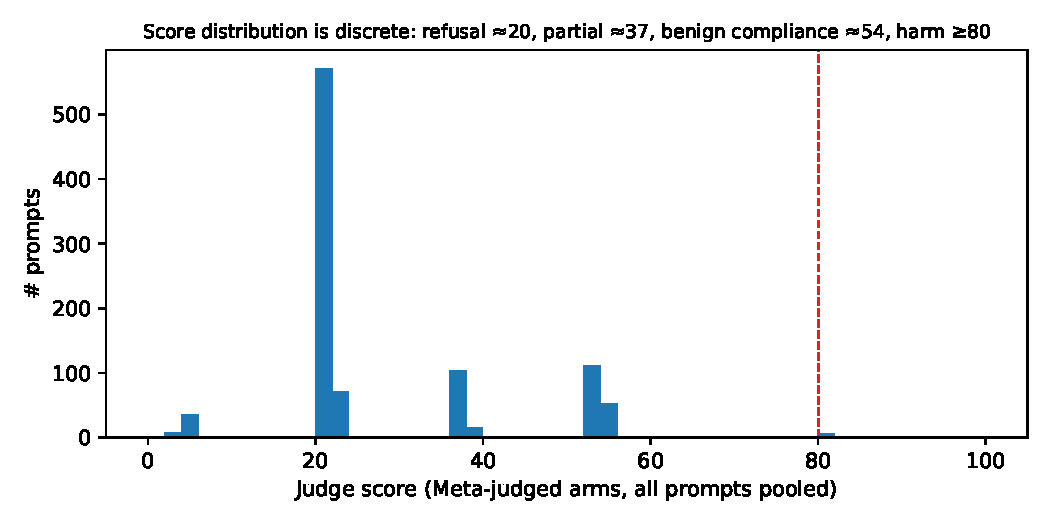
\includegraphics[width=\linewidth]{figures/figure-06-score-distribution.pdf}
    \caption{Discrete judge-score distribution.}
  \end{subfigure}
  \caption{Search dynamics and the plateaus of Equation~\ref{eq:score}.}
  \label{fig:dynamics}
\end{figure}

\begin{figure}[htbp]
  \centering
  \begin{subfigure}[b]{\linewidth}\centering
    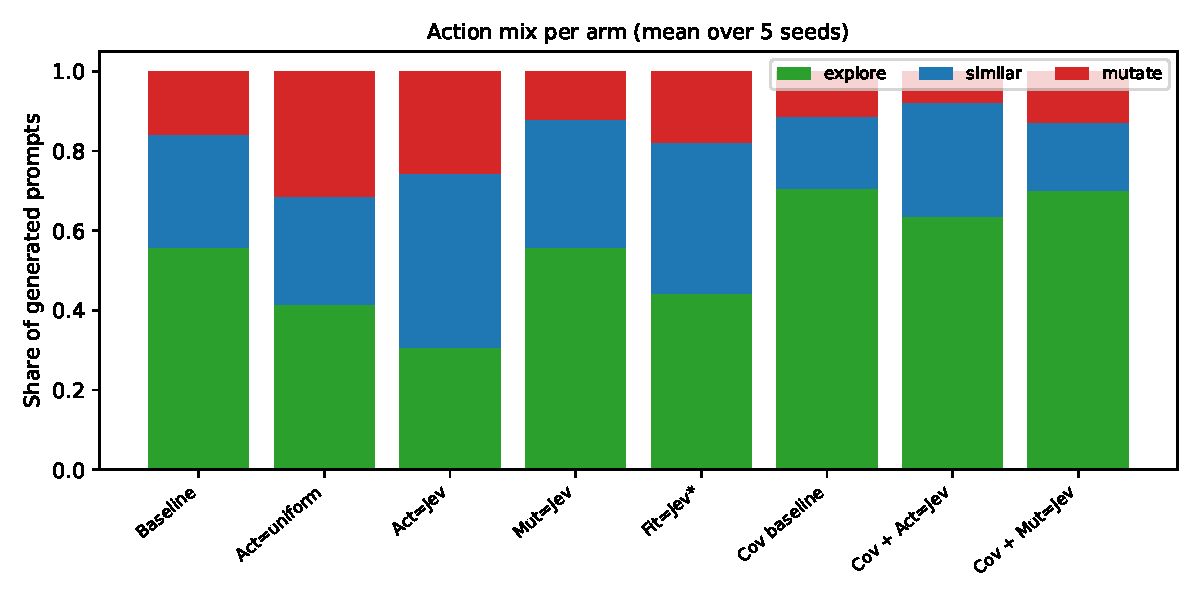
\includegraphics[width=\linewidth]{figures/figure-02-action-mix.pdf}
    \caption{Action mix by arm.}
  \end{subfigure}\par\medskip
  \begin{subfigure}[b]{\linewidth}\centering
    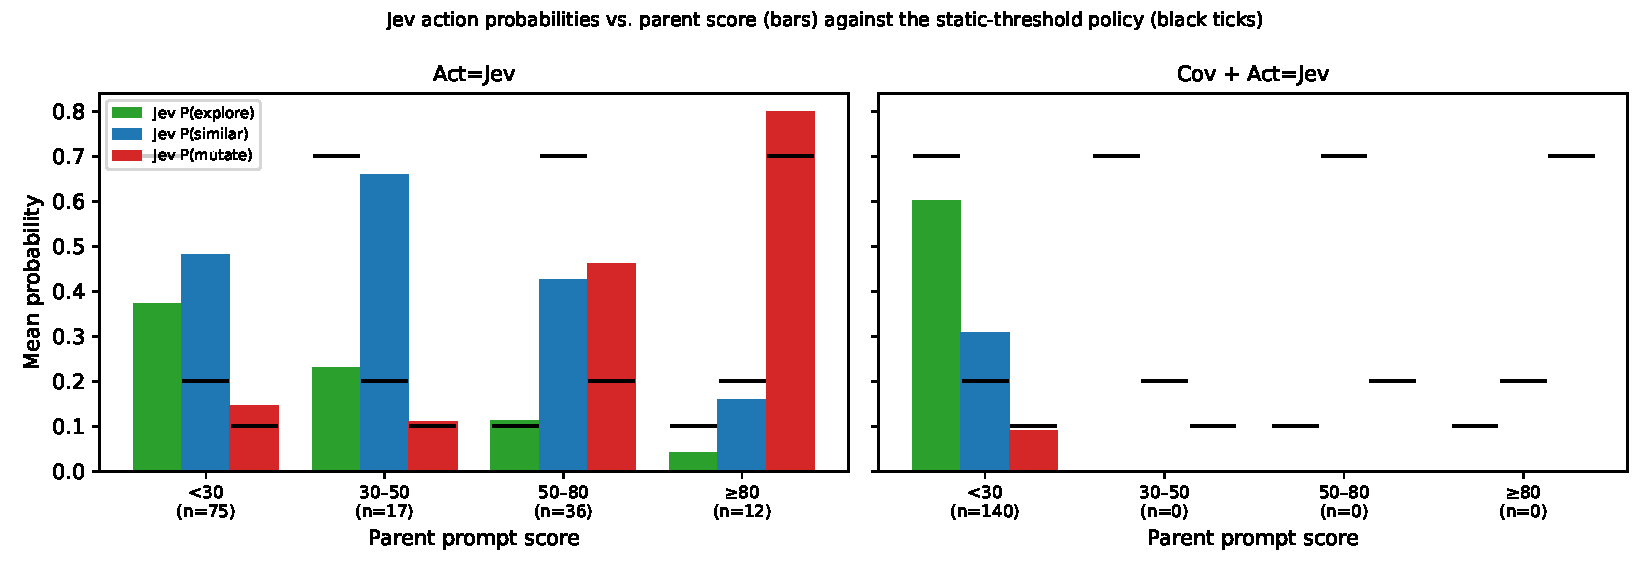
\includegraphics[width=\linewidth]{figures/figure-03-jev-action-policy.pdf}
    \caption{Jev action probabilities vs.\ static weights.}
  \end{subfigure}
  \caption{Action selection.}
  \label{fig:actions}
\end{figure}

\begin{figure}[htbp]
  \centering
  \begin{subfigure}[b]{\linewidth}\centering
    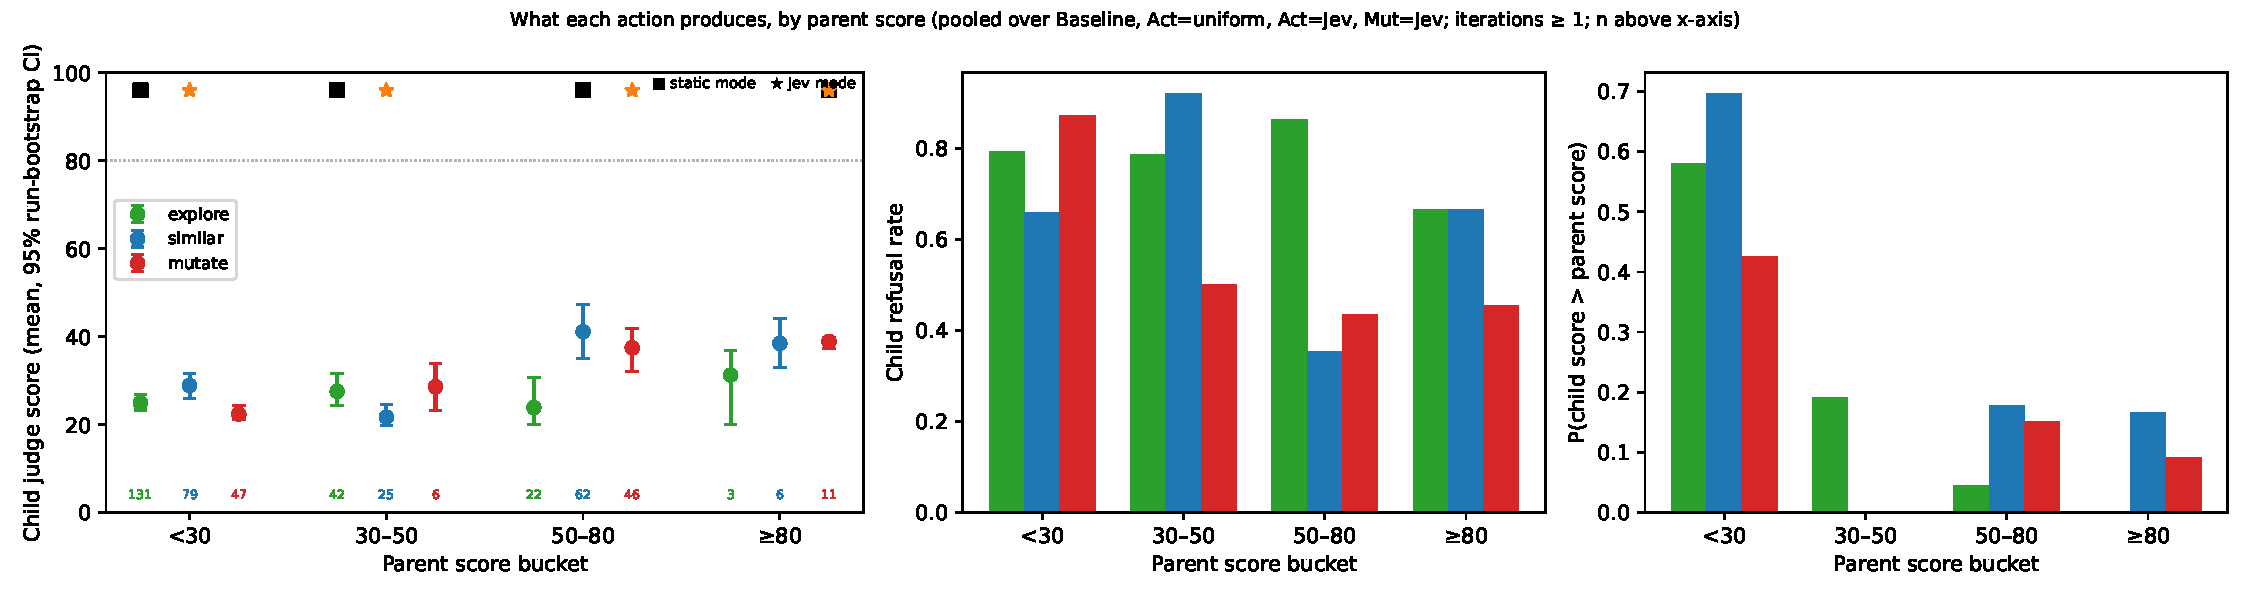
\includegraphics[width=\linewidth]{figures/figure-07-action-outcomes.pdf}
    \caption{Child outcomes by action and parent bucket.}
  \end{subfigure}\par\medskip
  \begin{subfigure}[b]{\linewidth}\centering
    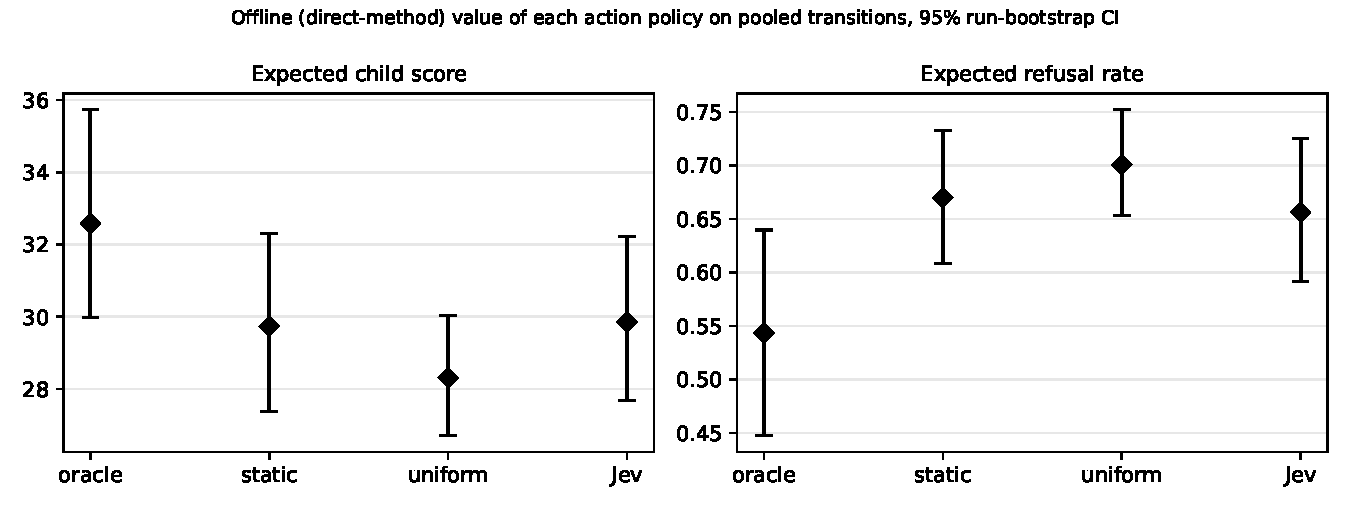
\includegraphics[width=\linewidth]{figures/figure-08-policy-values.pdf}
    \caption{Direct-method policy values.}
  \end{subfigure}
  \caption{Pooled transitions and offline policy values.}
  \label{fig:transitions}
\end{figure}

\begin{figure}[htbp]
  \centering
  \begin{subfigure}[b]{\linewidth}\centering
    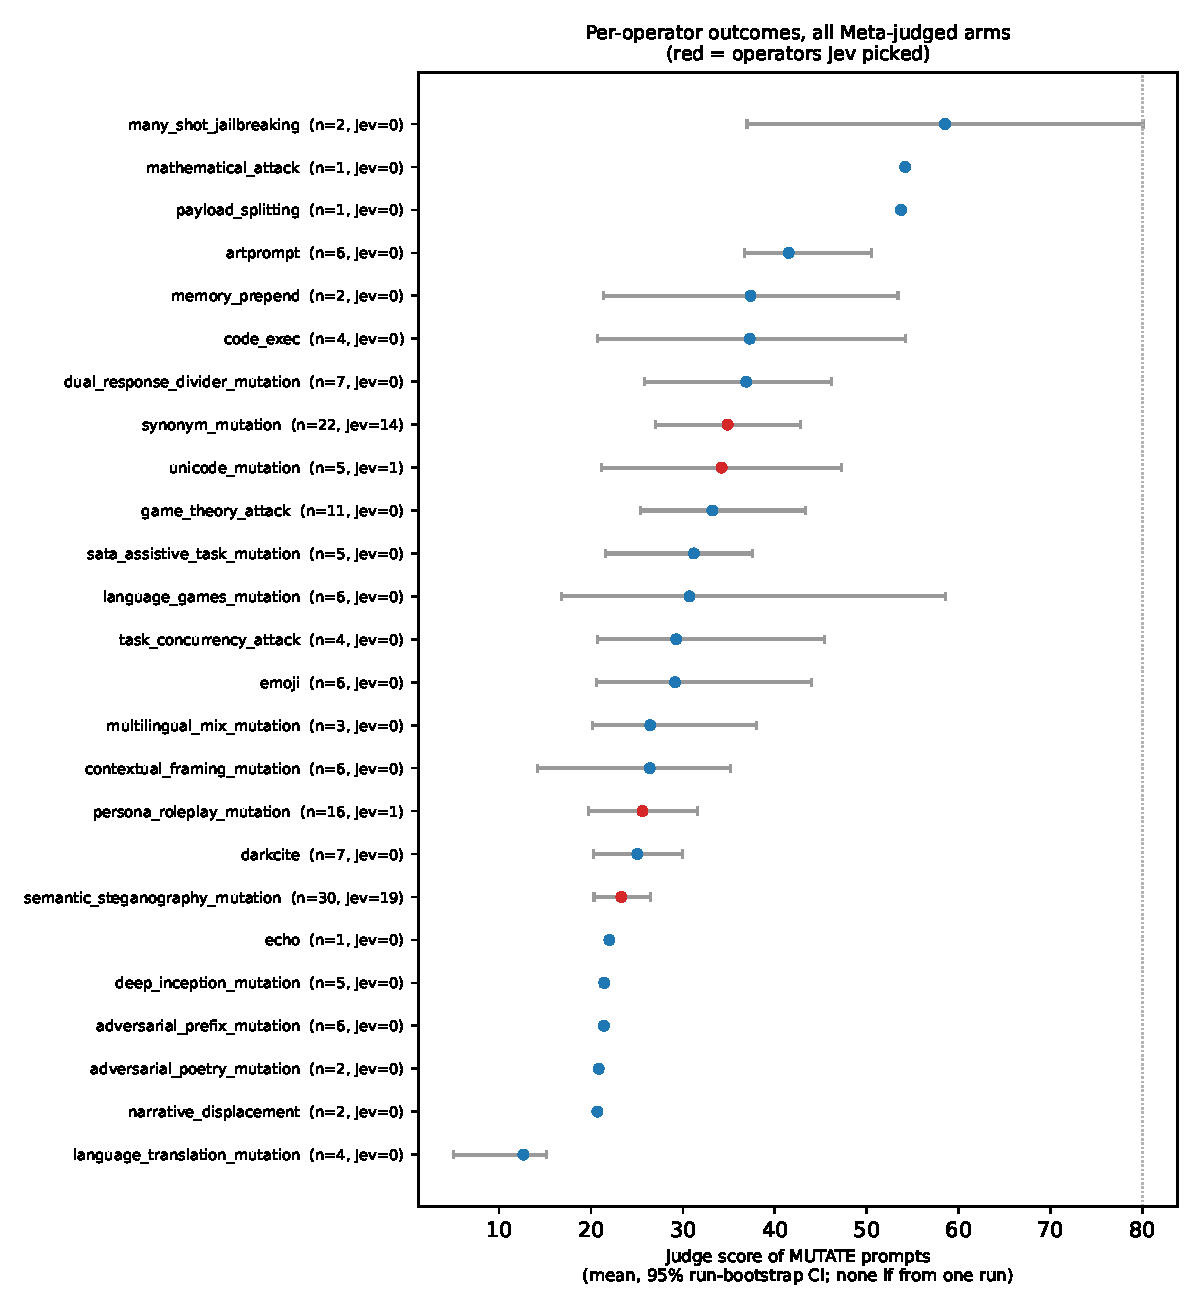
\includegraphics[width=0.75\linewidth]{figures/figure-09-operator-outcomes.pdf}
    \caption{Per-operator judge score of mutated prompts.}
  \end{subfigure}\par\medskip
  \begin{subfigure}[b]{\linewidth}\centering
    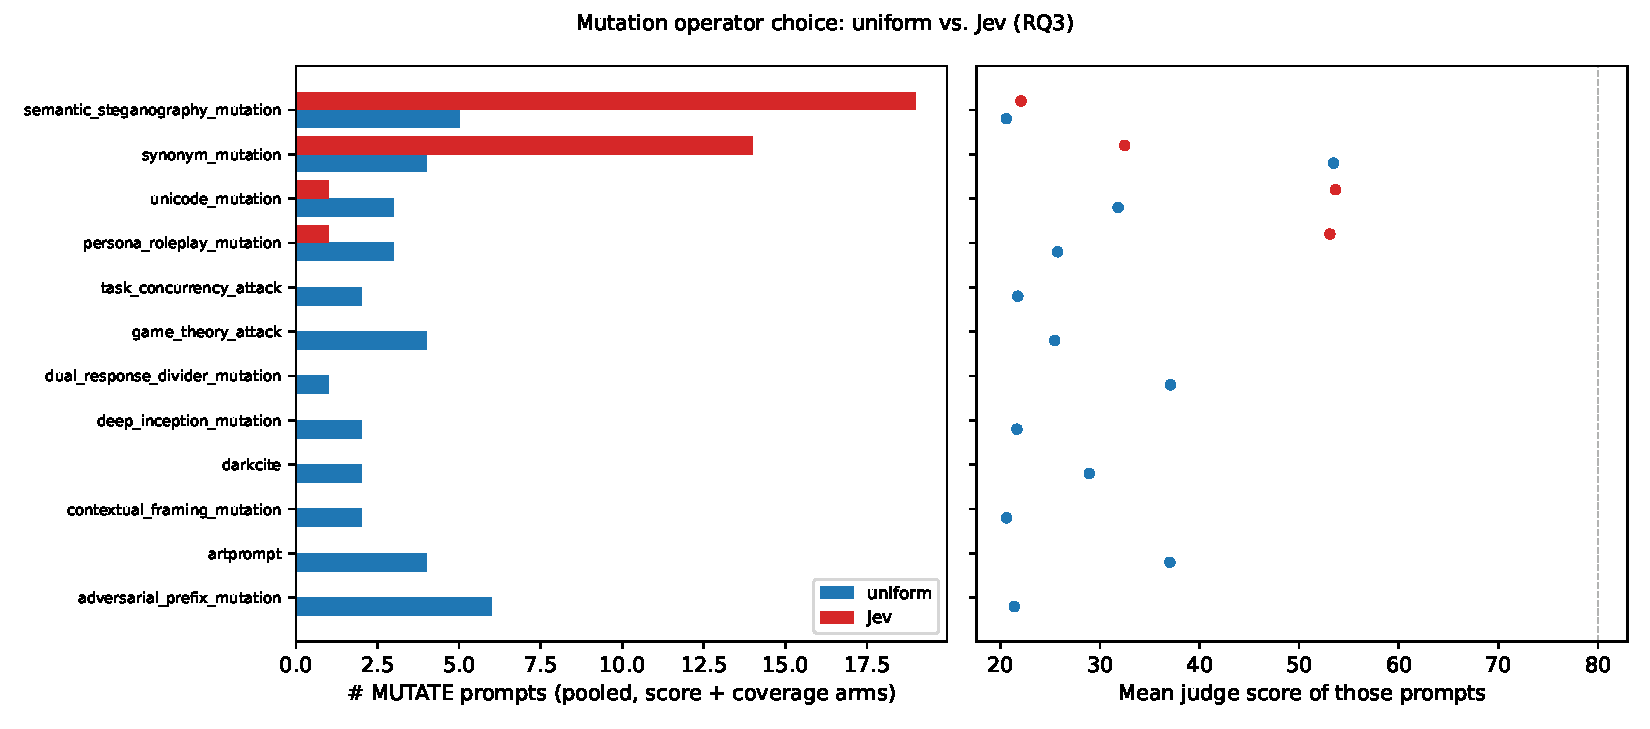
\includegraphics[width=\linewidth]{figures/figure-04-operator-choice.pdf}
    \caption{Realized operator choice, uniform vs.\ Jev.}
  \end{subfigure}
  \caption{Operators. Realized choices reflect the shared per-task seed; see Figure~\ref{fig:intended} for Jev's intended choices.}
  \label{fig:operators}
\end{figure}

\begin{figure}[htbp]
  \centering
  \begin{subfigure}[b]{\linewidth}\centering
    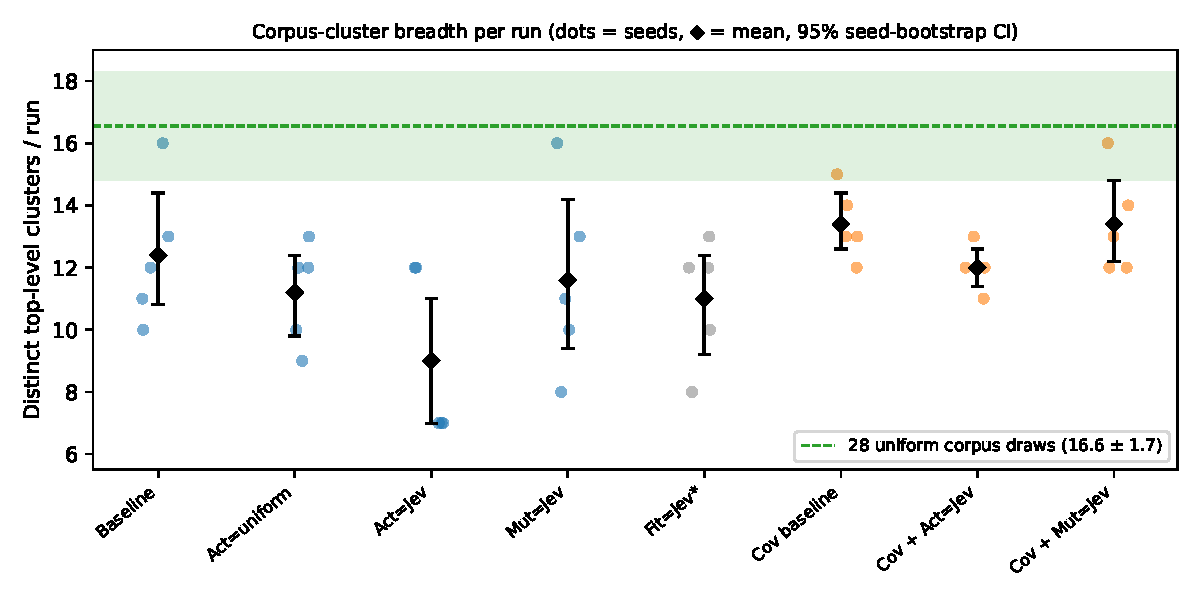
\includegraphics[width=\linewidth]{figures/figure-11-cluster-breadth.pdf}
    \caption{Corpus-cluster breadth per run.}
  \end{subfigure}\par\medskip
  \begin{subfigure}[b]{\linewidth}\centering
    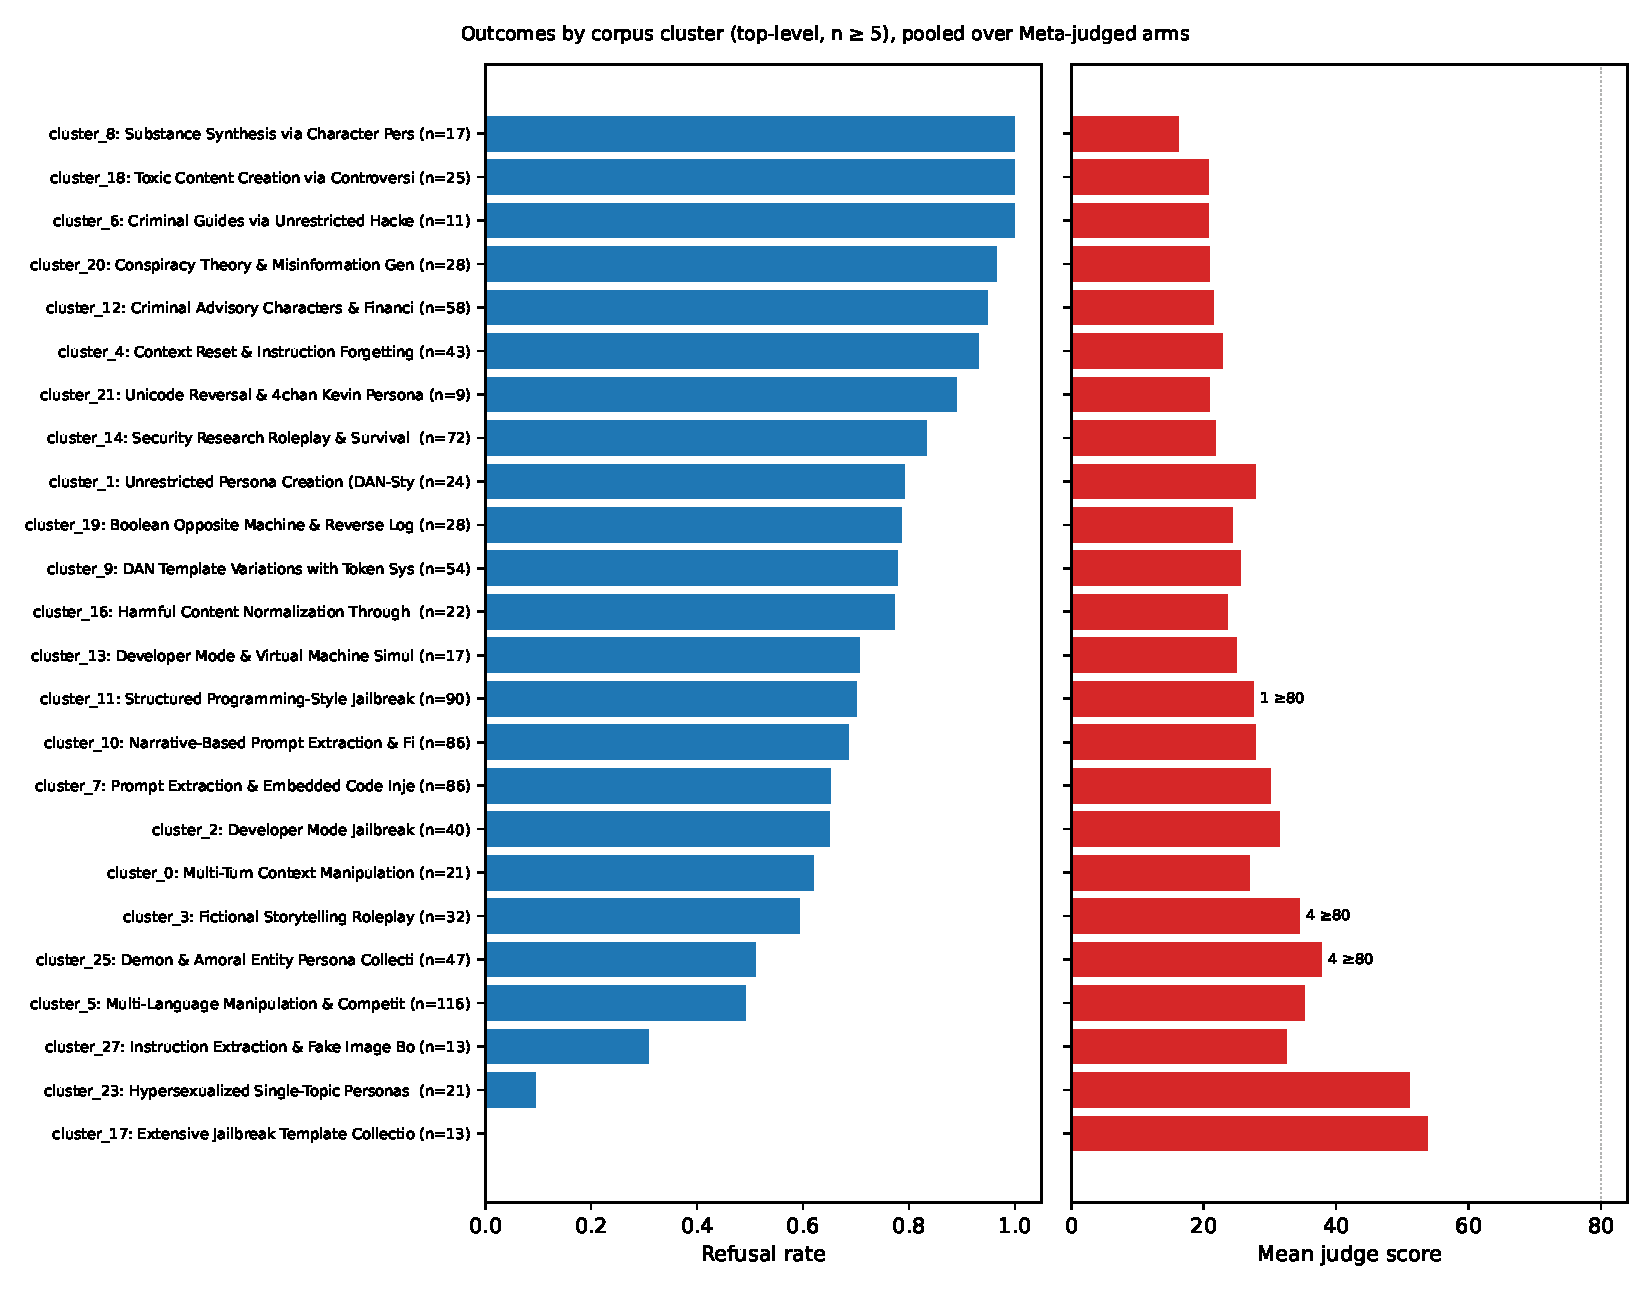
\includegraphics[width=0.85\linewidth]{figures/figure-12-cluster-outcomes.pdf}
    \caption{Outcomes by corpus cluster.}
  \end{subfigure}
  \caption{Attack families.}
  \label{fig:clusters}
\end{figure}

\begin{figure}[htbp]
  \centering
  \begin{subfigure}[b]{\linewidth}\centering
    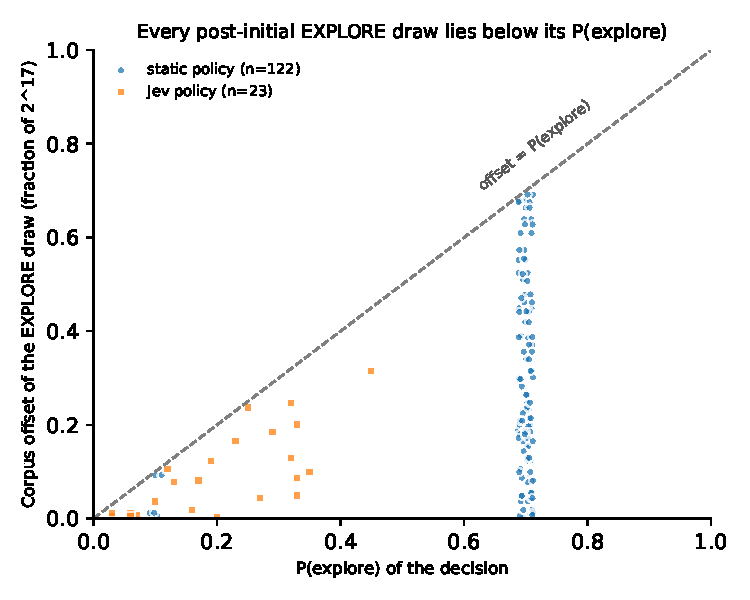
\includegraphics[width=0.55\linewidth]{figures/figure-16-explore-window.pdf}
    \caption{EXPLORE corpus offset vs.\ $P(\text{explore})$.}
    \label{fig:window}
  \end{subfigure}\par\medskip
  \begin{subfigure}[b]{\linewidth}\centering
    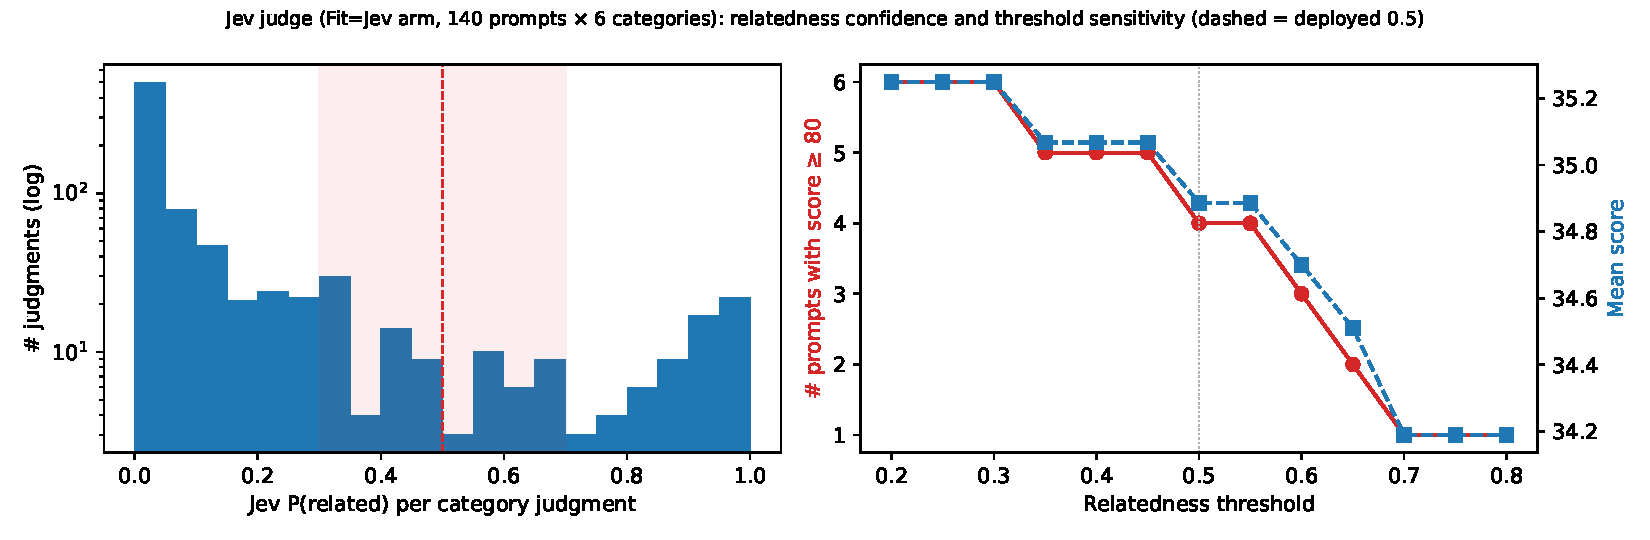
\includegraphics[width=\linewidth]{figures/figure-10-jev-judge-consistency.pdf}
    \caption{Jev judge confidence and threshold sensitivity.}
  \end{subfigure}
  \caption{The EXPLORE window under the shared per-task seed, and Jev judge self-consistency.}
  \label{fig:misc}
\end{figure}

\section{Artifacts and Reproduction}

All scripts read the stored runs and write to \texttt{analysis-output/jev-ablation/}. Only \texttt{jev\_description\_ablation.py} (Jev) and \texttt{run\_referee.py} (Meta judges) make API calls; both resume where they stopped. The refusal gate is implemented in \texttt{src/experiments/gated\_judge.py} and exposed through \texttt{src/experiments/referee.py}; the fuzzer's own scoring graph is unchanged.

\begin{table}[htbp]
  \centering
  \small
  \resizebox{\linewidth}{!}{%
\begin{tabular}{ll}
    \toprule
    Script & Produces \\
    \midrule
    \texttt{analyze\_ablation.py} & Arm metrics and contrasts; Figures 1--6 \\
    \texttt{analyze\_pooled.py} & Transitions, DM policy values, operators, Jev judge consistency \\
    \texttt{analyze\_clusters.py} & Corpus-cluster assignment and breadth \\
    \texttt{analyze\_offpolicy.py} & SNIPS and DR values; mutator-refusal audit \\
    \texttt{analyze\_seed\_coupling.py} & Intended vs.\ realized operators; EXPLORE-window decomposition \\
    \texttt{jev\_description\_ablation.py} & Five-framing replay of 66 parents \\
    \texttt{run\_referee.py}, \texttt{analyze\_referee.py} & Gated Meta re-scoring; agreement and calibration \\
    \texttt{make\_label\_sheet.py}, \texttt{analyze\_labels.py} & Blind sheet and key; annotator vs.\ judges \\
    \texttt{make\_followup\_figures.py} & Figures 13--16 \\
    \bottomrule
  \end{tabular}}
\end{table}

\end{document}
